% final.tex
% John Scott
% CS610 Spring 2019
% This work is mine unless otherwise cited.

% AllegThesis.tex
% by A. Thall
% 13 Feb 2003
%
% Revised by R. Roos
% Nov 2013
%
% This document provides a sample Senior Thesis template for use
% by students in Allegheny's CS and Applied Computing programs.
%   ********************************************************************
%   * BEGINNING OF PREAMBLE:                                           *
%   ********************************************************************

\NeedsTeXFormat{LaTeX2e}
\documentclass[12pt]{report}

%   ********************************************************************
%   * ALL BUT ONE OF THE FOLLOWING 5 LINES SHOULD BE COMMENTED OUT.    *
%   * (NOT ALL OF THESE OPTIONS HAVE BEEN TESTED IN THIS REVISION!)    *
%   ********************************************************************

%\usepackage[debug,draft,double]{gatorthesis} % for student proof doublespace
%\usepackage[bottom,double]{gatorthesis} % for final department copy
\usepackage[debug,draft,single]{gatorthesis} % for student workcopy
%\usepackage[single]{gatorthesis} % for student
%\usepackage[debug,draft,nolists,nofront,single]{gatorthesis} % more options


\usepackage{comment}     % provides a way to "comment out" sections in blocks
\usepackage{doublespace} % final document should be double-spaced!
\usepackage{amsmath}     % special symbols
\usepackage{amssymb}     % more special symbols
\usepackage{epsfig}      % needed for including figures
% \usepackage{fancybox}  % --- DISABLED BY RSR, SEP 2013 ---
\usepackage{url}
\usepackage{listings}
\usepackage[figure]{algorithm2e}
\usepackage{graphicx}

% EXAMPLE: Don't hyphenate the words "itself" or "linear". Hyphenate
%          "representations" only at the places indicated by the "-":

\hyphenation{itself repre-sen-tations linear}

% The following provides a box to surround the thesis statement
%\newenvironment{Thesis}%
%{\begin{Sbox}\begin{minipage}{.95\linewidth}}%
%{\end{minipage}\end{Sbox}\begin{center}\fbox{\TheSbox}\end{center}}

%   ********************************************************************
%   ********************************************************************
%   ***  END OF PREAMBLE.                                            ***
%   ********************************************************************
%   ********************************************************************



%   ********************************************************************
%   * DOCUMENT CONTENT STARTS AT THE "\begin{document}" COMMAND:       *
%   ********************************************************************
\flushbottom
\begin{document}

%   ********************************************************************
%   * FILL IN THE "{...}" BELOW WITH YOUR INFORMATION.                 *
%   ********************************************************************

\thesistitle{Scottipy: An In-Depth Playlist Creator/Editor Using the Spotify API}

\thesisauthor{John Scott} \thesisadvisor{Dr. Aravind Mohan}

\thesisnumber{CS2019-12} % SEE PAULINE LANZINE TO GET YOUR REPORT NUMBER!

\thesisreadera{Dr. Gregory Kapfhammer}


%   ********************************************************************
%   * IN RARE CASES YOU MAY HAVE MORE THAN TWO READERS, IN WHICH CASE  *
%   * YOU SHOULD UN-COMMENT THE FOLLOWING AND ADD NAMES:               *
%   ********************************************************************
% \thesisreaderb{Dr. Your Thirdreader}
% \thesisreaderc{Dr. Your Fourthreader}
% \thesisreaderd{Dr. Your Fifthreader}

%   ********************************************************************
%   * YOU MAY IGNORE THE FOLLOWING COMMAND:                            *
%   ********************************************************************
\date{\FileRevised \\ $\mbox{}$Revision: 1.8 $\mbox{}$}

\thesismaketitle         % Creates the title page
\thesismakecopyright     % Creates the copyright page

%   ********************************************************************
%   * YOU MAY SPLIT YOUR THESIS INTO SEVERAL FILES AND "\include" THEM *
%   * AS SHOWN BELOW. FOR INSTANCE, FILE "abstract.tex" CONTAINS THE   *
%   * ABSTRACT, FILE "ack.tex" CONTAINS THE ACKNOWLEDGMENTS, ETC. YOU  *
%   * MAY, OF COURSE, PUT EVERYTHING INTO ONE HUGE FILE, BUT THERE ARE *
%   * ADVANTAGES TO SPLITTING THINGS UP--FOR EXAMPLE, YOU CAN COMMENT  *
%   * OUT "\include" LINES OF SOME PARTS IN ORDER TO PRINT DRAFTS      *
%   * CONTAINING SELECTED SECTIONS OF YOUR THESIS, SAVING PAPER AND    *
%   * PRINTING COSTS.                                                  *
%   *                                                                  *
%   * YOU ARE NOT REQUIRED TO HAVE A "dedication"--IF YOU DON'T, JUST  *
%   * DELETE THAT LINE OR COMMENT IT OUT WITH A LEADING "%"            *
%   ********************************************************************

\begin{abstract}
Spotify collects hundreds of data points for every song in their massive catalog
of music. Information on features of the song, as well as meta-data about the
artist, can paint a near complete picture that can be analyzed and compared to
other songs. Despite this breadth of data, music discovery on Spotify is lacking
in many ways. Other than a single automatic and static weekly playlist, there is
no easy way to find new music related to a user's taste and preferences. This
thesis paper explores the creation of a web-based playlist creator and editor, dubbed
"Scottipy", using Spotipy, a Python wrapper for the official Spotify API. This project
seeks to extend the current boundaries of music personalization.
\end{abstract}
  % REQUIRED!

% \include{dedication} % OPTIONAL

\chapter*{Acknowledgements}

If I had to complete this on my own, I wouldn't have been able to. I first have
to thank my parents, as well of the rest of my family, for supporting me even when
I doubted myself. Thanks to Dr. Mohan and Dr. Kapfhammer, and all of my professors
and peers in the Allegheny Computer Science Department. Shouts out to my friends
and roommates, you kept me going. Special thanks to Jon Schaeffer and Zac Shaffer,
for the 11th hour bug squashing.
       % OPTIONAL, BUT ALMOST EVERYONE INCLUDES IT

%   ********************************************************************
%   * FRONT MATTER--TABLE OF CONTENTS, ETC. YOU PROBABLY DON'T NEED TO *
%   * CHANGE ANY OF THIS UNLESS YOU HAVE NO TABLES OR FIGURES, OR YOU  *
%   * WANT TO CHANGE NUMBERING DEPTH FOR SUBSECTIONS, OR ...           *
%   ********************************************************************

\setcounter{tocdepth}{2}    % # of section levels shown in table of contents
\setcounter{secnumdepth}{3} % # of numbered subsection levels in the text

\tableofcontents
%\listoftables       % OMIT THIS IF YOU DON'T HAVE ANY TABLES
\listoffigures      % OMIT THIS IF YOU DON'T HAVE ANY FIGURES

%   ********************************************************************
%   * A GLOSSARY IS ALMOST NEVER NEEDED UNLESS YOU HAVE AN UNUSUALLY   *
%   * LARGE NUMBER OF SPECIAL TERMS OR NOTATIONS AND IT WOULD DETRACT  *
%   * TOO MUCH FROM THE FLOW OF THE PAPER TO DEFINE THEM IN-LINE.      *
%   ********************************************************************
%\include{glossary}  % OMIT THIS IF YOU DON'T HAVE A GLOSSARY (FEW PEOPLE DO)


%   ********************************************************************
%   * THE FOLLOWING "lstset" COMMAND IS ADAPTED FROM ONE FOUND AT:     *
%   * http://tex.stackexchange.com/questions/115467/                   *
%   * listings-highlight-java-annotations                              *
%   *                                                                  *
%   * SEE CHAPTER 3 AND APPENDIX A                                     *
%   ********************************************************************

\lstset{
  basicstyle=\footnotesize\tt, % the size of the fonts that are used for the code
  breakatwhitespace=false,     % automatic breaks only happen at whitespace?
  breaklines=true,             % sets automatic line breaking
  captionpos=b,                % sets the caption-position to bottom
  frame=single,                % adds a frame around the code
  language=Java,               % the language of the code
  keywordstyle=\bf,
  showspaces=false,
  showstringspaces=false,      % underline spaces within strings only?
  showtabs=false,
  tabsize=2                    % sets default tabsize to 2 spaces
}

%   ********************************************************************
%   * NOW INCLUDE THE CHAPTER FILES; COMMENT OUT ANY YOU DON'T WANT TO *
%   * PROCESS IN A PARTICULAR LATEX RUN.                               *
%   *                                                                  *
%   * INCLUDED FILES ARE ASSUMED TO END IN ".tex", E.G.,               *
%   * "ch01_overview.tex", "ch02_relatedwork.tex", ETC.                *
%   ********************************************************************

% ch:intro
%
% $Id: ch01_overview
%
%   *******************************************************************
%   * SEE THE MAIN FILE "AllegThesis.tex" FOR MORE INFORMATION.       *
%   *******************************************************************

\chapter{Introduction}\label{ch:intro} % we can refer to chapter by the label

The Spotify API allows public access to an ever-growing list of end points
for every song in their 40 million and growing music catalog. Despite this vast
wealth of information, Spotify users are not allowed to select tracks based on this
data. This chapter lists the driving motivations for this project, analyzes other
ventures into Spotify API data, and outlines the goals and vision for this
application.
\section{Motivation} \label{sec:motivation}

The personal motivations for this project stemmed from a series of criteria that
I wanted my thesis to fulfil, before choosing a specific project to pursue. The
requirements included:
\begin{itemize}
  \item Inclusion of music - As an active musician at Allegheny College, as well
  as a music theory minor, it almost went without saying that I wanted to include
  my biggest passion in a senior research project.

  \item Practicality - I sought to create a project that, at the very least, could
  likely have continued real-world utilization by myself (and hopefully others)
  after the conclusion of my academic career.

  \item Opportunity to learn - Being not well-versed in working with existing APIs,
  as well as the area of both front-end and back-end web development, I saw this
  assignment as an opportunity to explore areas I was not able to through college
  courses
\end{itemize}

Apart from these self-defined criteria, after settling on the specific topic of playlist
creation, the Spotify API itself served as motivation. My simultaneous amazement of
the power that Spotify holds, as well as frustration for the lack of use and support
of the breadth of data generated, was enough to begin creating a tool to remedy
this shortfall in music discovery.

Spotify currently controls 36\% of the global music streaming market \cite{Midia:18}. With a
catalog of well over 40 million songs, there is an abundance of music to fit
any listeners' taste. Despite this, Spotify has no easy way to use the information
Spotify collects to sort and choose songs, other than a selection of premade playlists
for diferent genres and keywords. Artist pages include tabs categorizing related artists,
but there is no way to quickly generate a list of songs that
takes advantage of the track information Spotify possesses. The Spotify
API can allow for this and much more, but curated music discovery is limited to one weekly
playlist, called "Discover Weekly", consisting of 30 songs tailor made for each
Spotify user. As accurate as this playlist is, it merely scratches the surface of
what the data that Spotify possesses can achieve. With so much more data on every
song in Spotify's library already available, the motivation for this project is
simple: allowing Spotify customers to find new music at any time, with any selected
specifications, puts the power of discovery in their hands. Finding new songs is
always enjoyable, and this project can create that feeling at a user's disposal.


\section{Current State of the Art}\label{sec:stateofart}

In 2014, Spotify acquired the music intelligence company "The Echo Nest" \cite{echo:14}.
The company collects hundreds of data points on songs, such as values for the key,
tempo, song duration, time signature, and other features. They have also created
formulas to calculate more abstract features, including energy and "danceability".
These values are composites of simpler points; energy is based on overall loudness
of a song, as well as segment duration, which refers to loops and repeated sections
of songs. The danceability formula has not been released, but is a combination of
beat strength, tempo and tempo stability, and other undisclosed factors. Spotify
gaining control of the company gave them access to this database, and a year later
the Discover Weekly playlist was released \cite{Constine:15}.

The Discover Weekly playlist is so successful because of the way it is tailored to
Spotify customers. The first deciding portion is pulled from the user's
"taste profile", aggregated from songs a user listens to, or saves to their library.
The profile is grouped into clusters, such as this example for reporter Nikhil Sonnad
\cite{Pasick:15}:

\begin{center}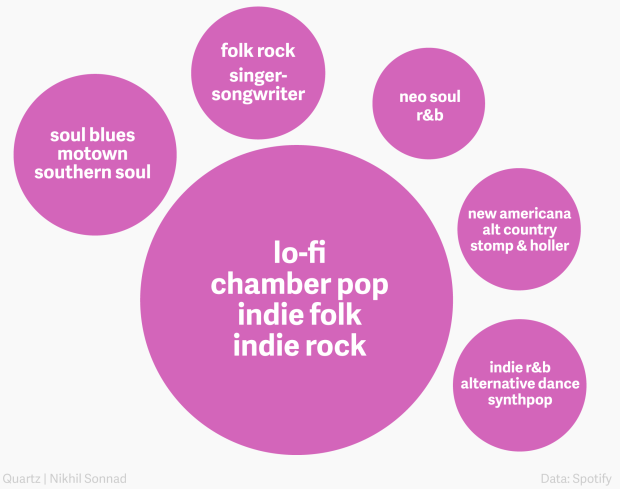
\includegraphics[height=6cm]{images/cluster-genres.png}

\end{center} Fine-grained genres, such as "chamber pop", or "stomp \& holler", are taken from
methods from The Echo Nest, and are used as a first level of personalization. The cluster-based
approach serves to eliminate many songs that users will not be interested in, but also allow
multiple wide-spanning genres that may have no relation with each other.

The other prong of the Discover Weekly method is collaborative filtering \cite{Ciocca:17}. For
Spotify, this technique works by comparing users who have played many of the same tracks in
the same genre. Spotify creates a giant matrix to compare the songs, with each row corresponding
to one of the 140 million users, and a column for each song in their catalog \cite{Spotify:15}.
\begin{center}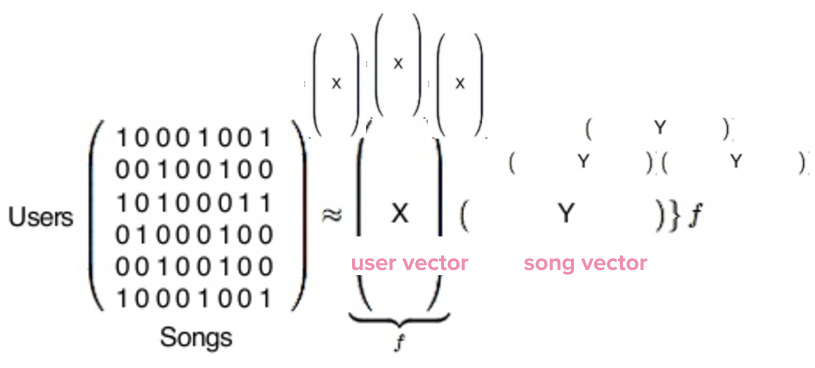
\includegraphics[height=6cm]{images/matrix.png}

\end{center} The user vectors, represented by columns in the matrix, are compared
with each other to find their closest matches, determined by similar patterns of
interactions with the same tracks. Songs which appear
in user's A's vector, but not in user B's, are recommended to user B. The end
result is a playlist of music which feels handpicked by a close friend, but is
actually the result of a cleverly crafted algorithm. Currently, the Discover Weekly
playlist is the gold standard for personalized music discovery. Millions of users
receive a list of songs they are likely to enjoy, every week without fail.

\section{Goals of the Project}\label{sec:goals}

As this project is an academic thesis, and not just a simple weekend hobby, my
overarching objective is to demonstrate what I have been able to learn at
Allegheny College, as a capstone to end my academics. More specifically to this
tool, I wish to prove my ability to meld my passion of music, with my major of
computer science. In this process, I wish to research utilization of established,
robust APIs, to create an application that shows principles which can be brought
with me into the professional industry. Upon beginning this thesis project, I have
just elementary experience on working with APIs, and even less knowledge of web
development. With these shortcomings in mind, my primary goal in completing this
thesis is to develop a working ability in these areas as such:

\begin{itemize}
  \item Spotify API - be able to call information from Spotify's database, in a
  way which allows music listeners greater control over tracks they listen to.

  \item Web Development - Explore front-end and back-end web development strategies,
  as well as the use of framework and bootstrap tools, to package my tool in a more
  logical and accessible way for public use.
\end{itemize}

Concerning goals within the scope of the tool, the objective of this project is
to create a web-based application which allows music fans of all levels to create
fine-tuned playlists, based on any amount of available criteria. As previously
discussed, the Discover Weekly playlist is the premier tool for finding song
tracks unrecognized to the user. However, the tool has its own set of drawbacks.
Since both methods use Spotify customer behavior to create parameters, non-subscribers
will not be able to use the feature at all, and less active or new subscribers will
not have a baseline for the technique to begin from. In addition, the playlist
only refreshes once a week, giving thirty new tracks. There is no way to manually
reset your playlist, or get more new songs. The project I outline would be web-based,
using the data that Spotify already possesses. Using the Spotify
API, I will create a custom playlist which could be played in the page, or saved to a user's
profile. The input for the tool would be any song in the Spotify catalog, or alternatively
genres or certain keywords. Keywords would be words that appear in popular playlist titles,
and tracks would be selected from them. In addition to this user input, there will also be
options to adjust ranges of features that are inherent to every song, such as overall song
popularity, tempo, energy, amount of vocals present, and other characteristics. These metrics
allow fans to fine tune the resulting playlist, ensuring they will be able to find enjoyable
tracks, making finding new songs an easy task for any music fan.

Considering this project heavily involves something I am passionate about, I foresee
myself adding features, and increasing the robustness of this application, for years
to come down the road. The Spotify API is constantly adding features and increasing
available information, so the final state of this project is apt to change after
the conclusion of the academic year. Because of this possibility, it is important
that I do not lose track of the scope and time available. Especially for areas I
have less experience with, success may be defined as having a working "proof of
concept", and a fully functional web-app may have to be completed at a later time.
My final goal is to enjoy the process of creating a working product, which should
be aided by the subject matter.

\section{Thesis Statement}\label{sec:statement}

This thesis project is an application stemming heavily from research into the
Spotify API, as well as various strategies utilized for hosting the playlist
creator and editor methods in a web-app. The resulting product will be designed
to allow any user to edit and create Spotify playlists, taking advantage of the
end points of tracks in the Spotify catalog. The target audience is music fans
of any level of theory knowledge, so making the application both usable and accessible
for anyone is a major design concern. Research into the Spotify API will directly
impact the design and output of the project.

\section{Thesis Outline}\label{sec:outline}

Chapter \ref{ch:music} outlines the idea of Music Information Retrieval, as well as how the
field has been used in existing Spotify projects. Chapter \ref{ch:method} gives a framework of
how the Spotify API is structured, as well as outlines of Spotipy and Flask. Chapter
\ref{ch:implem} outlines the initial design of the project, including specific code
examples to better explain the product. Chapter \ref{ch:conclusion} lists future
improvements that are desired, as well as new conceptual features.
 % Introduction -- of course, you can name it anything!

% ch:music
%
% $Id: ch02_music
%
%   *******************************************************************
%   * SEE THE MAIN FILE "AllegThesis.tex" FOR MORE INFORMATION.       *
%   *******************************************************************
\chapter{Related Work}\label{ch:music}

This chapter gives a description of what music information retrieval (MIR) is, as well as how
the data has been used by Spotify services, as well as third parties using the Spotify API.
Other applications using the Spotify API are also outlined, and compared to Scottipy.

\section{Music Information Retrieval}
One of the first overviews on MIR \cite{Downie:03} uses seven pieces of information
to analyze each song. These areas are pitch, tempo, harmony, timbre, as well as
editorial information, lyrics, and bibliographic information. The pitch of a song
includes notes, intervals between notes, as well as key. The temporal facet included
the speed of a song, time signature, and pitch and harmonic duration. Harmony refers
to two or more pitches at the same time creating a polyphony of notes. This area
also includes chords and chord progressions. The timbral area includes tone color,
such as the difference in sound quality between a flute and a violin. Orchestration,
or instrument selection, is the most important part of timbre. The editorial section
is mostly performance instructions on music, such as notes for dynamics and
articulations. The textual facet is the lyrics of a piece. The lyrics viewed alone
are usually a good measure of the mood of a song, though they may not be enough to
find a desired melody. The paper mentions an example of this phenomenon between
"God Save the Queen" and "My Country 'tis of Thee", as two songs with the same
melody but different lyrics. The bibliographical facet has little to do with the
actual form of the song, but more meta information about who made the song. This
can include:
\begin{itemize}
  \item song title
  \item composer
  \item arranger
  \item editor
  \item performer
\end{itemize}
and other descriptions about a song, rather than traits garnered from the song. Although these
seven facets include all of the information needed about a song, for comparison purposes a more
nuanced look at individual areas within these groupings would be needed. The paper also includes
looks into systems that use MIR, which can be grouped into either analytic/production, or locating
systems. Analytic and production services focus mostly on the complete digital representation of
music, with a deemphasis on bibliographical information. Projects like this are used to create
comprehensive theoretic analyses of songs. Locating systems are used to quickly retrieve existing
works, such as finding songs based on user criteria and where they can be played.

\section{MIR in Spotify}
The Spotify API offers many different features for songs, which include "danceability",
energy, key, loudness, mode, "speechiness", "acousticness", "instrumentalness", duration,
time signature, "liveness", valence, and tempo \cite{Dev:18}. In addition to the data points mentioned
earlier, Spotify uses many others from The Echo Nest to paint a portrait of a musical
composition. Danceability, valence, energy, and tempo
are all different ways of measuring the mood of a track, typically songs with a happier
mood will have higher values. Loudness, speechiness, and instrumentalness are all properties
of songs, showing how much of a given element is present.  Liveness and acousticness show the
context of a song, so if it is a live recording or an acoustic version.

\section{Related Works}

The Spotify Developer Showcase \cite{Spotify:19} is a collection of submitted
projects that take advantage of various facets of the Spotify API. Since the
API collects information about user listening habits, as well as song data, many
projects focus on using existing user data. One such project is Klarafy
\cite{DeBock:17}, which takes information from a user's playlists, to find
classical music that they are more likely to enjoy. Klarafy's documentation states,

\begin{quote}
Klarafy starts from the relatively plausible premise that someone who loves loud,
fierce metal, is more likely to enjoy a loud, fierce piece by Wagner than soft,
delicate piano music. Klarafy seeks out the affinities, similarities or
connections between your favourite music and classical music.
To arrive at this 'translation', Klarafy scans your playlist for three criteria:
- your favourite music genre (most common genre);
- the musical mood that prevails in your playlist;
- points of departure determined in advance, such as specific instruments,
voice types, etc.
\end{quote}

Klarafy aggregates data from user playlists, and links that data to a
predetermined set of composers and their works. There is no way to get a new
artist if your taste doesn't fit the composer, however, and getting a new
emotion would practically  involve resetting your Spotify profile.

musicScape \cite{Aleksik:18} is another example relying on user data, which
takes recently played tracks for a user, to generate a minimalist landscape from
audio features of the songs. The color and landscape will change, based on track
features from recently played music.

\begin{center}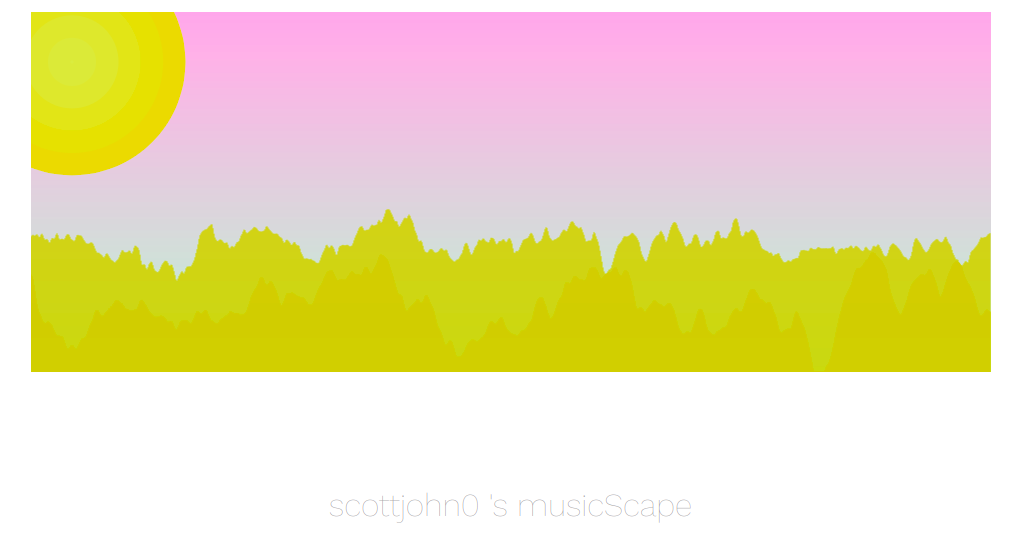
\includegraphics[height=7cm]{images/musicScape.png}
\end{center}

Playlist Souffle \cite{Hammer:18} is another playlist editor, but it works by
swapping out songs in a playlist, and replacing them with tracks either from the
same album, or by the same artist. This tool can be useful to find lesser-known
songs, while still having a connection to songs the user enjoys.

\begin{center}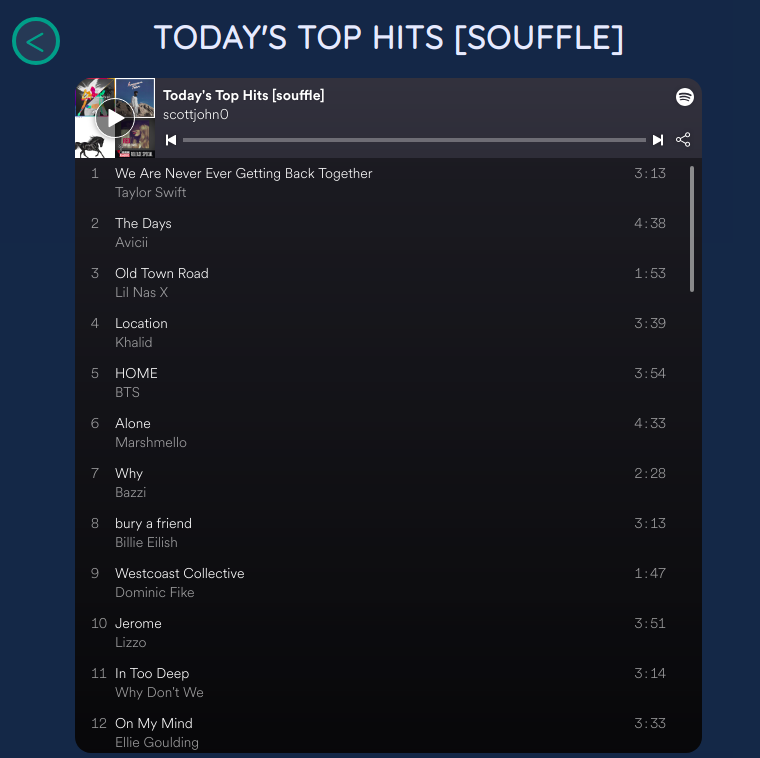
\includegraphics[height=7cm]{images/souffle.png}
\end{center}

The above image is a "souffle" seeded from Spotify's "Today's Top Hits" playlist
\cite{TopHits:19}. The songs have all been changed out, but there is no other
manipulation that can be done. Because of this, the tool is limited as a
"one-and-done", that can only be so effective at finding new music.


Since the spirit of this project is to allow the general public to use the strength
of Spotify's library, and not just established users, projects that do not rely on
user profile data can be more comparable to Scottipy. One of these is MagicPlaylist
\cite{Magic:15}, which is also a web-based playlist creator. The site is much more
limited in its usage of Spotify song data, however; a look through the GitHub source
page \cite{Lovera:15} shows that resulting playlists are based on one aspect of
Spotify artist pages, which is the related artist feature. Because of this,
creating multiple playlists using songs from the same artist as a seed will
give near identical results. In addition to this drawback, there is no way to
edit the resulting list of songs. In tandem, these design decisions create a
rather static experience, which leaves a lot to be desired in terms of creating
an enjoyable collection of music.

Although there are many services using various parts of Spotify's API, no publicly
showcased projects can create playlists based on user chosen criteria, and make
a dynamic result. In the next chapters, I outline how Scottipy seeks to create
a program that meets these challenges.
 % Background, literature survey, ...

% ch:method
%
% $Id: ch03_thework.tex
%
%   *******************************************************************
%   * SEE THE MAIN FILE "AllegThesis.tex" FOR MORE INFORMATION.       *
%   *******************************************************************
%
\chapter{Method of Approach} \label{ch:method}
This chapter outlines how the process of building the project will work. It also
shows how the Spotify API works, and includes an outline of Spotipy and Flask.

\section{User Inputs}

The existing Spotify API allows for searching for tracks, albums, artists, and playlists, which
makes it easy for the user to enter a song name and quickly find it. For example, here is a query
for the term "dark fantasy":
\\

\lstset{language=Java}
\begin{lstlisting}
curl -X "GET" "https://api.spotify.com/v1/search?q=dark%20fantasy&type=track" -H "Accept: application/json"
-H "Content-Type: application/json"
\end{lstlisting}

The result is the Spotify link to the track, as well as information about the popularity,
and listing on its album.\\

\begin{lstlisting}
"href": "https://api.spotify.com/v1/tracks/7yNK27ZTpHew0c55VvIJgm",
        "id": "7yNK27ZTpHew0c55VvIJgm",
        "is_local": false,
        "name": "Dark Fantasy",
        "popularity": 66,
        "preview_url": null,
        "track_number": 1,
        "type": "track",
        "uri": "spotify:track:7yNK27ZTpHew0c55VvIJgm"
\end{lstlisting}

From the previous step, information about the song can be found by searching for its audio features:
\\
\begin{lstlisting}
curl -X "GET" "https://api.spotify.com/v1/audio-features/7yNK27ZTpHew0c55VvIJgm"
-H "Accept: application/json" -H "Content-Type: application/json"
\end{lstlisting}


This query results in an easy to use list of characteristics and their matching values:
\\

\begin{lstlisting}
{
  "danceability": 0.59,
  "energy": 0.587,
  "key": 5,
  "loudness": -5.919,
  "mode": 1,
  "speechiness": 0.0457,
  "acousticness": 0.274,
  "instrumentalness": 0,
  "liveness": 0.167,
  "valence": 0.367,
  "tempo": 88.015,
  "type": "audio_features",
  "id": "7yNK27ZTpHew0c55VvIJgm",
  "uri": "spotify:track:7yNK27ZTpHew0c55VvIJgm",
  "track_href": "https://api.spotify.com/v1/tracks/7yNK27ZTpHew0c55VvIJgm",
  "analysis_url": "https://api.spotify.com/v1/audio-analysis/7yNK27ZTpHew0c55VvIJgm",
  "duration_ms": 280787,
  "time_signature": 4
}
\end{lstlisting}

Each of the listed features can be compared to the rest of the Spotify library
to find similar tracks. In addition to tracks, keywords such as moods or events
would also be accepted as inputs. Instead of searching for tracks in that case, the
Spotify API allows us to find popular playlists with the keywords in the title.
In this example, the term "sleep" is queried, with no other context:
//

\begin{lstlisting}
curl -X "GET" "https://api.spotify.com/v1/search?q=sleep&type=playlist" -H "Accept:
application/json" -H "Content-Type: application/json"
\end{lstlisting}

This search finds the playlist called "Sleep", curated by Spotify, as the first result:
\\
\begin{lstlisting}
{
  "playlists": {
    "href": "https://api.spotify.com/v1/search?query=sleep&type=playlist&market=US&offset=0&limit=20",
    "items": [
      {
        "collaborative": false,
        "external_urls": {
          "spotify": "https://open.spotify.com/playlist/37i9dQZF1DWZd79rJ6a7lp"
        },
        "href": "https://api.spotify.com/v1/playlists/37i9dQZF1DWZd79rJ6a7lp",
        "id": "37i9dQZF1DWZd79rJ6a7lp",
        "images": [
          {
            "height": 300,
            "url": "https://i.scdn.co/image/f499b0497289a6432dcccfb6de5f57164739d525",
            "width": 300
          }
        ],
        "name": "Sleep",
        "owner": {
          "display_name": "Spotify",
          "external_urls": {
            "spotify": "https://open.spotify.com/user/spotify"
          },
          "href": "https://api.spotify.com/v1/users/spotify",
          "id": "spotify",
          "type": "user",
          "uri": "spotify:user:spotify"
        },
        "primary_color": null,
        "public": null,
        "snapshot_id": "MTU0MDkxNDI1OCwwMDAwMDBhNDAwMDAw
                    MTY2YzExYTAyNTcwMDAwMDE2MmYyYjBlOGQ4",
        "tracks": {
          "href": "https://api.spotify.com/v1/playlists/37i9dQZF1DWZd79rJ6a7lp/tracks",
          "total": 152
        },
        "type": "playlist",
        "uri": "spotify:user:spotify:playlist:37i9dQZF1DWZd79rJ6a7lp"
      },
\end{lstlisting}

Popular tracks from those would be added to the playlist created by this application.
Thus, the basis of the model can find related tracks from a user entering either a
song name, or even just an emotion that they would like to relate music to.

\section{Spotipy}

Spotipy is a \textit{Python} wrapper for the Spotify API, developed by The Echo Nest
team \cite{Lamere:17}. Spotipy gives full access to the data available from the
Spotify platform. Spotify's native resource identifiers, URL links, and IDs for
artists, tracks, playlists, and albums are all supported. Spotipy allows users to
quickly gather information such as recently played songs, saved tracks, playlists,
and albums, top played artists and songs, and even currently playing tracks.
There are also methods for featured playlists across Spotify, new releases, and
even recommendations from seed artists, genres, or tracks.

The track end points are listed below, with their types, value ranges, and descriptions.
\begin{itemize}
  \item Acousticness - float - 0.0 to 1.0 - Lack of electric sounds/instruments
  \item Danceability - float - 0.0 to 1.0 - Combination of tempo, rhythm stability,
  and beat strength
  \item Energy - float - 0.0 to 1.0 - Intensity, dynamic range, loudness, timbre, entropy
  \item Instrumentalness - float - 0.0 to 1.0 - Lack of vocals
  \item Liveness - float - 0.0 to 1.0 - If a track was performed live
  \item Loudness - float - -60 to 0 - Overall volume
  \item Speechiness - float - 0.0 to 1.0 - Presence of spoken words
  \item Tempo - float - 0 to 320 - Beats per minute of a track
  \item Valence - float - 0.0 to 1.0 - Musical positiveness of a track
\end{itemize}

Spotipy was chosen for this project simply for ease of use, and my own familiarity
with \textit{Python}, instead of using \textit{JavaScript}. This also allowed
coding to be quickly checked in the terminal, which in the testing process
was easier for me than using \textit{JavaScript}. From the beginning of the
research project to the present, I have not seen any advantage in using the native
API instead of Spotipy. From accessing the database, to general ease of use, Spotipy
had no visible limitations.

\section{Flask}
The flipside of coding in \textit{Python} rather than \textit{JavaScript}, was
the increased difficulty in creating a web app. Luckily, the Flask framework covered every need
of this project. Flask's emphasis on being a "micro framework" means that
\begin{quote}
By default, Flask does not include a database abstraction layer, form validation
or anything else where different libraries already exist that can handle that.
Instead, Flask supports extensions to add such functionality to your application
as if it was implemented in Flask itself. Numerous extensions provide database
integration, form validation, upload handling, various open authentication
technologies, and more \cite{Pallets:18}.
\end{quote}

Since the project does not currently require any advanced or complicated techniques,
a simpler framework like Flask can easily and smoothly handle the requirements.
In addition to these benefits, Flask has a strong online presence, and extensive
documentation. This became even more useful than I first realized, as it helped
me to create the HTML templates with more guidance than many other, perhaps more
robust, frameworks. The command line interface also included above average debugging,
which became quite useful in the learning process, even when my issues were in the
HTML templates, rather than the \textit{Python} source code. As this program grows
in the future, I will surely explore using other frameworks, if Flask becomes
limiting in features or speed. Django has become a likely choice, as I had the
opportunity to work with it in class this semester.
 % Chapter organization is topic-dependent

%ch:implem
%
% $Id: ch04_implementation.tex
%
%   *******************************************************************
%   * SEE THE MAIN FILE "AllegThesis.tex" FOR MORE INFORMATION.       *
%   *******************************************************************
%
\chapter{Implementation}\label{ch:implem}
This chapter outlines the design of the project. The packages and resources outlined
in the previous chapter are referenced in how they were used in the project design.
Many of the methods from the source code are outlined and explained, in order of how
they may be accessed by a user.

\section{Main Menu}
Due to time constraints of the thesis, much of this project still currently exists
as \textit{Python} scripts, which execute in the terminal. As such, to start the
project, the user must execute in the terminal.
\begin{lstlisting}[language=bash]
  $ python3 main.py
\end{lstlisting}

The \textit{main.py} serves only as a gateway to the two current scripts,
\textit{recent.py} and \textit{edit.py}. The available input options are "recent",
"edit", and "exit". The entire script is encompassed in a while loop, such that
an incorrect input simply prompt the user for another input. The function scripts
are called using: \begin{verbatim} exec(open("./file.py").read()) \end{verbatim}

\section{Playlist Editor}
\textit{edit.py} is used to edit a user's existing playlists by filtering them
using the Spotipy API data. As outlined in the previous chapter, this project uses
the Spotipy wrapper for the official API, written in JavaScript. The constructor
function (Figure 4.1) is used for user authentication; the \texttt{CLIENT\_ID},
\texttt{CLIENT\_SECRET}, \texttt{REDIRECT\_URI},
and SCOPE variables are all needed for any projects that use the Spotify API.

\pagebreak
\begin{figure}
\begin{lstlisting}[aboveskip=0pt]
  def __init__(self):
    self.CLIENT_ID = SPOTIPY_CLIENT_ID
    self.CLIENT_SECRET = SPOTIPY_CLIENT_SECRET
    self.REDIRECT_URI = "http://localhost:5000"
    self.SCOPE = "playlist-read-private playlist-modify-private
    playlist-read-collaborative
    playlist-modify-public"
    self.sp = self.getUser() #Creates Spotify instance
    self.id = self.sp.me()["id"] #Gets ID of authenticating user
\end{lstlisting}
\caption{{\tt edit.py} constructor}
\end{figure}

Once the user is authenticated, the \textit{getPlaylist} function (Figure 4.2) gets the name
of every playlist the user has created or followed on Spotify. It also assigns
a numeric value to each one.


\begin{figure}
\begin{lstlisting}[aboveskip=5pt]
  def getPlaylist(self):
    #This function gets all playlists from the user.
    results = self.sp.current_user_playlists()
    for i, item in enumerate(results["items"]):
      print ("{number} {name}".format(number=i, name=item["name"]))
\end{lstlisting}
\caption{{\tt edit.py getPlaylist} function}
\end{figure}

The user then inputs the corresponding number to the playlist they desire to
filter. On the selection, a series of graphs are generated, illustrating the
distribution of the editable end points of songs in the playlist. When the user
closes these plots, they are prompted to enter the low and high values of the
end points of the tracks, in the \textit{getLimits} function. Leaving the input
empty will automatically choose the lowest and highest possible values for each
set, so if a certain criteria doesn't matter, no songs will be excluded by it.

The \textit{getSongs} function is then triggered, which
returns the song IDs for every track in the playlist. Once the track IDs are
gathered, the song features are returned using the \textit{getFeatures} function.
Thanks to Spotipy, this takes only a single line of code. (Figure 4.3)

\begin{figure}[!h]
\begin{lstlisting}
def getFeatures(self, track):
  #This function retrieves audio features from Spotify
  features = self.sp.audio_features(track)
  return features
\end{lstlisting}
\caption{{\tt edit.py getFeatures} function}
\end{figure}

It is at this point that the API end points are utilized, in the \textit{sortSongs}
function. In a series of nested \textit{if} statements, each desired range is
checked for each value of the songs. If they all return true, the song "passes",
and is added to the generated playlist. The \textit{createPlaylist} function
takes the passing songs, and creates a playlist using two Spotipy methods:
\textit{user\_playlist\_create} and \textit{user\_playlist\_add\_tracks}.
At this point, plots with an identical format as generated from the initial playlist
are once again created, in order to concretely visualize the new changes. The final
line to execute opens the user's playlists in a web page, using the \textit{open\_new\_tab}
method from the \textit{webbrowser} package. This puts the user one click away from
the newly generated playlist.

\section{Web Interface}
The \textit{recent.py} file is a venture into creating a web portal, using the Flask
framework to facilitate the use of \textit{Python}, as outlined in the previous
chapter. Initialized similarly to \textit{edit.py}, the authorization process
is nearly identical, but with more robustness. Upon either creation or discovery
of the authentication token, the Flask app will first return the last 50 tracks
the user has saved to their profile, using the \textit{current\_user\_saved\_tracks}
method. Unfortunately, the Spotify API limits rates to 50 per call, but an if statement
paired with a dynamic offset in the \textit{getSongList} function allows this
number to be increased, albeit with a very miniscule cooldown time.

\begin{figure}[!h]
\begin{lstlisting}
if callNo == 0:
        offset = 0
    else:
        offset = callNo*min(playlistLength, 50)

    results = sp.current_user_saved_tracks(limit=min(playlistLength, 50), offset=offset)
\end{lstlisting}
\caption{Dynamic Offset}
\end{figure}


The app then opens an HTML template. The user is
presented with a form, in which they may choose to create a Spotify playlist,
with options for the number of songs, a limit to the number of songs by a single
artist, and whether the playlist should be shuffled or not. (Figure 4.5)

\begin{figure}[!h]
\begin{lstlisting}
<div>
    <form action="/run" method="POST">
    Number of songs: <br>
    <input type="number" name="playlistLength" value="50" min=20>
    <br><br>
    Max songs per artist: <br>
    <input type="number" name="maxSongs" value="3" min=1>
    <br><br>
    <input type="checkbox" name="shuffle" value="True">Shuffle Songs?
    <br><br>
    <input type="submit" value="Create Playlist!" autofocus>
    </form>
</div>
\end{lstlisting}
\caption{{\tt runRecentlyadded.html} input form}
\end{figure}



These values are passed into a thread in the \textit{run} function, which then
loads the \textit{running.html} page.

\begin{figure}[!h]
\begin{lstlisting}
<div>
    <h3>Generating playlist. Please wait...</h3>
    <progress value= {{ progress }} max="100"></progress>
</div>
\end{lstlisting}
\caption{{\tt running.html} progress bar}
\end{figure}

The \textit{running.html} is mainly a placeholder, but does include a progress
bar corresponding to the creation of the playlist (Figure 4.6).

In order to limit the maximum number of songs from a single artist, the code needed
the ability to generate \textit{r} random, sorted integers from [0, n). This method
was taken from an example by Raymond Hettinger \cite{Hettinger:04} (Figure 4.7).

After removing the excess songs, the playlist is created and populated, using
a similar method to \textit{edit.py}. On generation of the playlist, the user
is redirected to the \textit{success.html} template, which has options to view
the created playlist on Spotify's web player, and to go back to the input form.


\begin{figure}[!h]
\begin{lstlisting}
def sample(n, r):
    #taken from http://code.activestate.com/recipes/272884-random-samples-without-replacement/
    #Generate r randomly chosen, sorted integers from [0,n)
    rand = random.random
    pop = n
    for samp in range(r, 0, -1):
        cumprob = 1.0
        x = rand()
        while x < cumprob:
            cumprob -= cumprob * samp / pop
            pop -= 1
        yield n-pop-1
\end{lstlisting}
\caption{Hettinger's random generator}
\end{figure}

\clearpage

\section{Result Testing}

In order to empirically check the effectiveness of the playlist editing, the
Matplotlib library for Python \cite{Matplotlib:19} was used to generate graphs
showing the values of the audio features, before and after the editing process.
In addition to this, the "pandas" library \cite{Pandas:19} was used to create a
dataframe with the track data.


\begin{figure}[!h]
\begin{lstlisting}
  ax1 = fig2.add_subplot(331)
  ax1.set_xlabel('Danceability')
  ax1.set_ylabel('Count')
  ax1.set_title('Danceability Distribution')
  pos_dance.hist(alpha= 0.5, bins=30)
  ax2 = fig2.add_subplot(331)
  neg_dance.hist(alpha= 0.5, bins=30)
\end{lstlisting}
\caption{Plot Template}
\end{figure}

As seen above, eight graphs are generated, one for each available end point. The
graphs show the distribution of the end point values, as well as the amount of
tracks that have each value.

\begin{center}
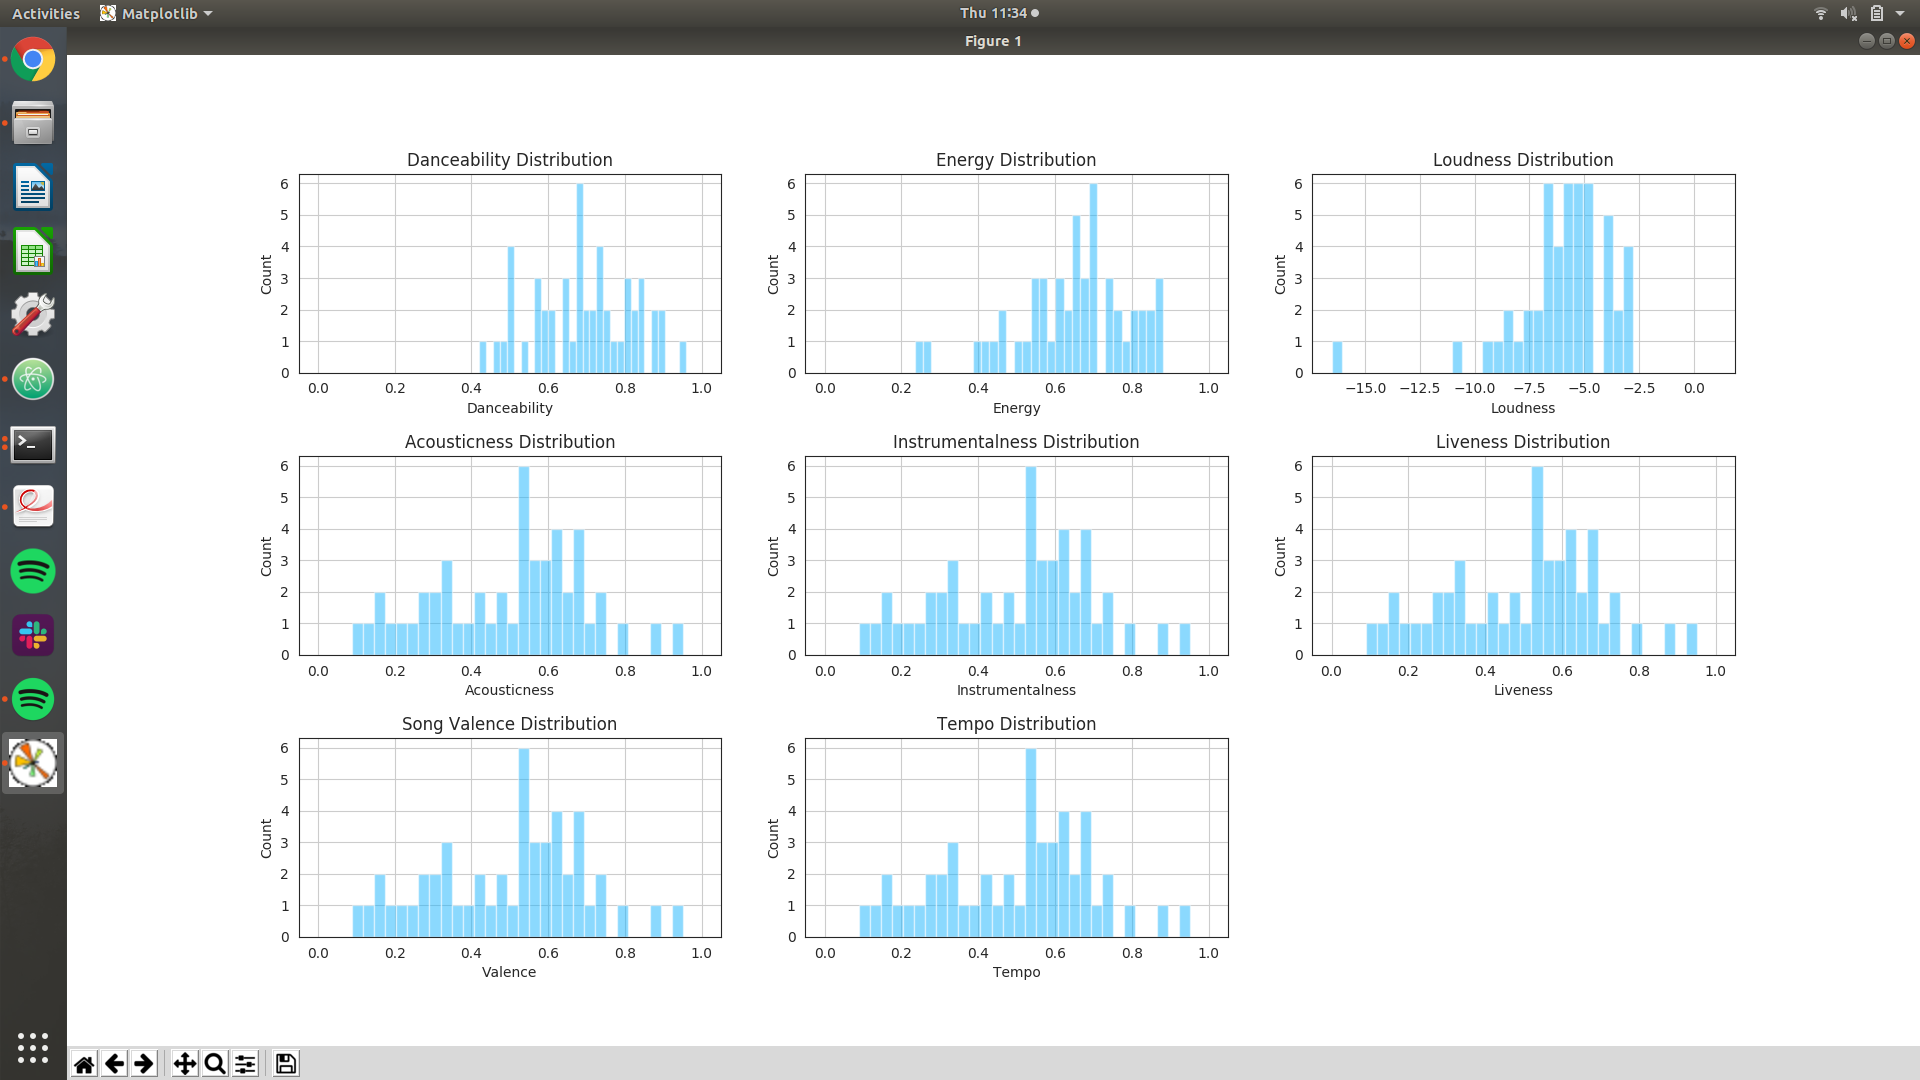
\includegraphics[height=8cm]{images/before.png}
\end{center}

The above graphs are generated from Spotify's "Today's Top Hits" playlist
\cite{Spotify:19}, which consists of the current 50 most popular songs in
Spotify's catalog. The values are reflective of current pop music, with a
heavy skew towards high energy music, which is also danceable. Interestingly,
valence is fairly evenly distributed, suggesting that some of the tracks subject
matters are sadder and more negative, but are still able to sound energetic
and danceable.

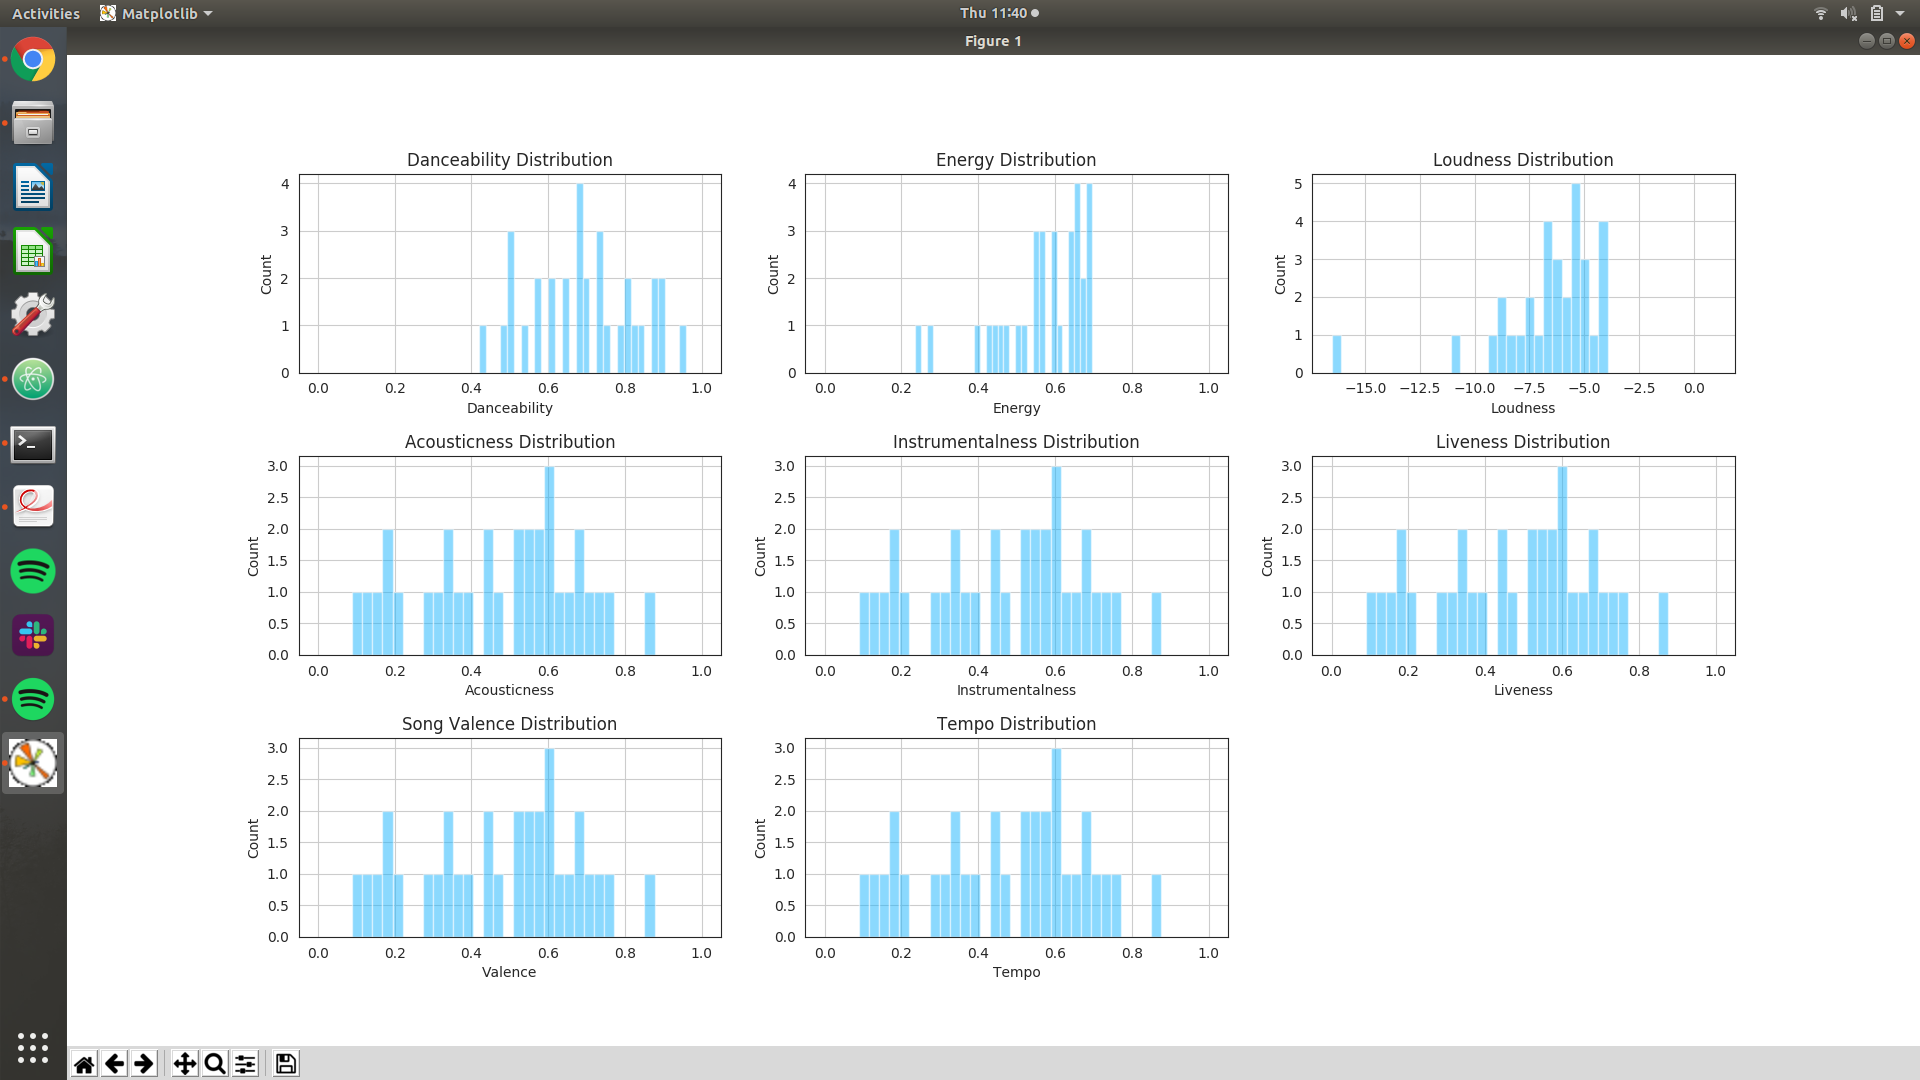
\includegraphics[height=8cm]{images/after.png}

These resulting graphs were aggregated from a playlist generated from "Today's Top Hits"
\cite{TopHits:19}, with the only applied requirement being energy less than 0.7.
Of course, the energy of the new playlist abruptly stops at .7, but the interesting
part is how several other end points are affected by this change. Loudness distribution
is limited to below -3.5 dB, which suggests that loudness is a major segment of the
formula used to calculate energy.

\section{Playlist Creation Efficiency}

\begin{figure}[!htb]
\begin{lstlisting}
if danceL <= songF["danceability"] <= danceH:
  if energyL <= songF["energy"] <= energyH:
    if loudL <= songF["loudness"] <= loudH:
      if acousticL <= songF["acousticness"] <= acousticH:
        if instrumentL <= songF["instrumentalness"] <= instrumentH:
          if livenessL <= songF["liveness"] <= livenessH:
            if valenceL <= songF["valence"] <= valenceH:
              if tempoL <= songF["tempo"] <= tempoH:
                return True
\end{lstlisting}
\caption{The sortSongs function}
\end{figure}

Due to the design of the function used to pick out songs that match the user
criteria, the playlist generation is the most time consuming element of the
program, most notably when applying to long playlists. Because of this, the
execution of each end point was measured, using the "time" Python library. This
was an attempt to see if the different endpoints took longer to sort than others,
and if the sorting process execution time was affected at all by the user defined
range of values. The Spotify-curated "Today's Top Hits" playlist \cite{TopHits:19}
was used to check each value. The first trials involved changing the ranges one
end point at a time, which resulted in a negligble amount of difference in
execution time for every variable. The next testing method was to attempt shrinking
the range of every variable simultaneously, compared to leaving every range
completely open. These changes also failed to create any noticeable difference
in execution time. This is likely due to the calls to the Spotify database,
which store the end points as identical types. Unless a more efficient way to
rewrite this method's code is found, the time to generate a playlist likely
will not be lowered. The execution time is limited by the necessary API calls,
which limits time optimization.

\section{Feasibility}
Due to the intrinsically subjective nature of music, graphical representations
which show that the playlist filtering is correctly working is not enough to
ensure that the resulting songs form an enjoyable listening experience. To this
end, the best testing method would involve human trials. Currently, I am the
only person to somewhat formally verify the correctness of the results, but
there are several avenues to allow more user feedback, which will likely be
pursued after the web portal is more complete. The first would be to simply
host the app on a web server, with a feedback form available for all users.
Questions relating to the user experience, and more specific inquiries about
satisfaction and accuracy of results would be valuable in tuning the metrics
for future use. Something as simple as a Google form could be used, with
questions including:
\begin{itemize}
  \item Did the application work correctly?
  \item Was the creator easy to use?
  \item How much, if any, music theory background do you have?
  \item Were you satisfied with the resulting songs?
  \item Were there any unwanted songs in the new playlist?
\end{itemize}
This feedback would be useful to gather another, outside perspective from my
own, hopefully making the project more accessible to any user.
Another available resource is the Spotify Developer Showcase
\cite{Spotify:19}, which features user developed projects built using the
Spotify API. Submitting Scottipy to the showcase would be another effective
way to increase the project's user base. These will be used after completing
the web portion of the project.
 % Chapter organization is topic-dependent

% YOU MAY HAVE SEVERAL MORE CHAPTERS, DEPENDING ON TOPIC AND ORGANIZATION

%ch:conclusion
%
% $Id: conclusion.tex
%
%   *******************************************************************
%   * SEE THE MAIN FILE "AllegThesis.tex" FOR MORE INFORMATION.       *
%   *******************************************************************
%

\chapter{Discussion and Future Work}\label{ch:conclusion}
This chapter outlines how the current state of the project compares to the original
proposal, including shortcomings and changes in the vision. It finishes with a reflection
on the application.

\section{Future Work}
The vision I have for the final version of this application is far beyond what
I was able to accomplish in one semester. I would like to eventually create a
fully functional web app, with a variety of options in the hopes of using as
much of the Spotify API as possible.

Due to the time constraints associated with this thesis project, the current
release is lacking many features that I expect the final application to include.
The biggest compromise was in the web page user interface, as I did not have the
time to configure every file to work with the Flask framework. Despite this, I am
encouraged that my first attempt works correctly, which should serve to make
future work easier, or at the least more familiar. If this project is to be used
by the general public, it is a necessity to be hosted on a website, with a user
interface that is both easy to understand and use. For this reason, creating an
entirely web-based application is the most pressing change to work on in the future.

Due to the structure of this project, it is conducive to add new features, without
having to weaken the integrity of the overall project. As such, the next feature
I would like to add is to trawl playlists for songs, by requesting a keyword from
the user. This would allow users to just type in a word, and receive songs that
other users have put in playlists related to the term. Since playlists are a
major part of Spotify, and contain songs chosen by users, instead of algorithms
alone, this is a powerful resource, which arrives pre-sorted. Therefore, choosing
songs from playlists will likely add a level of accuracy, and likeliness of
enjoyment, that is difficult to replicate by automation alone.

Another feature which I consider very important, especially for public use, is
mobile support. Again due to time, I did not have the opportunity to look into how
to develop for mobile, but I did learn that Flask can be used for mobile app
back-end. This is also encouraging for the final stage of this project. Like
much of the current internet, Spotify relies heavily on mobile usage. This is an
area I would like Scottipy to be able to access and address, but will require more
work.

A more conceptual change to investigate is to investigate Spotify user behavior,
in order to match this project with how users treat Spotify. In a paper focused
on this user behavior, user trends, and differences between desktop and mobile
usage were found \cite{6566767}. For one, the research team found that desktop
and mobile sessions peaked at different times through the day, and also in
different amounts; where destop sessions tended to peak higher than mobile, in
terms of percentage of total Spotify users.

\begin{center}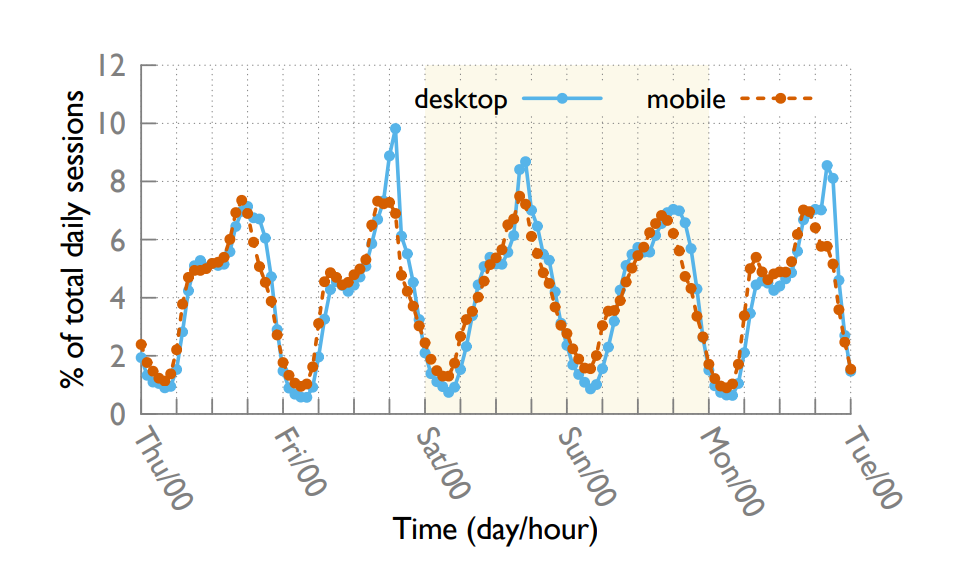
\includegraphics[height=9cm]{images/trends.png}
\end{center}

These tendencies of mobile users preceding desktop sessions were attributed by
the researchers to the number of commuting mobile users. This information may
be useful for Scottipy's mobile support, as it would suggest that the mobile view
should be very simple, while remaining robust in terms of available adjustable
options.

The research team also investigated the average session length of users, both
mobile and desktop. The team used Weibull distribution parameters to measure the
trends, where $\lambda$ and $\kappa$ are respectively the shape and scale of the
parameters.

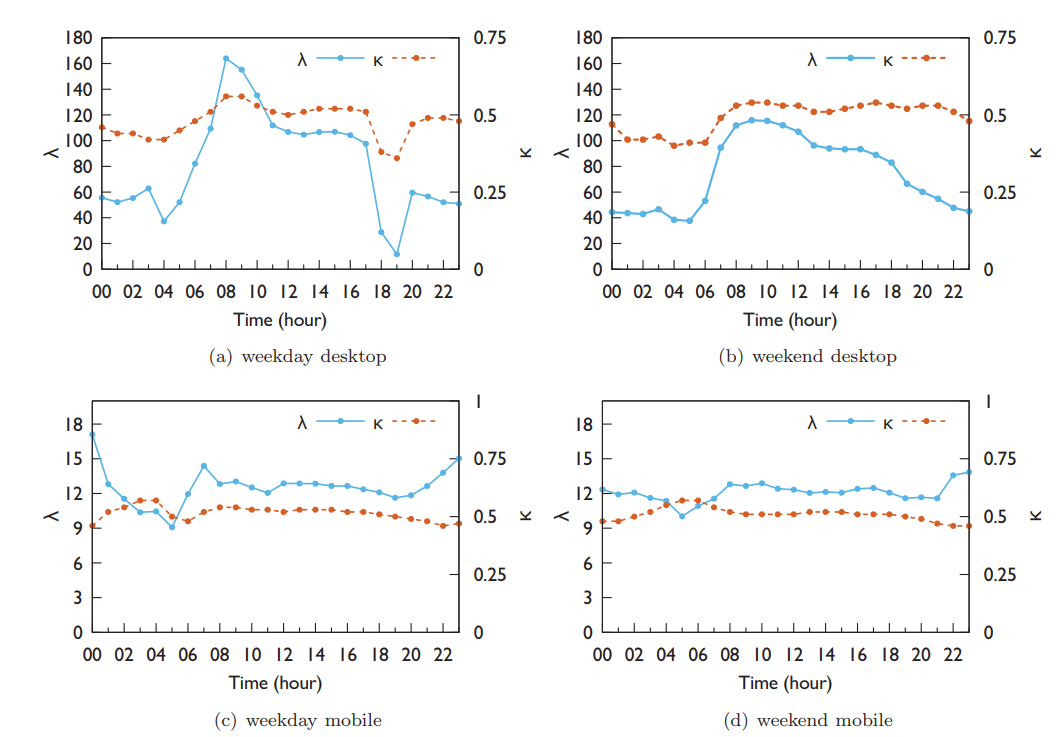
\includegraphics[height=9cm]{images/length.png}

The graphs above reveal much information about listening habits. In graph (a),
which is for desktop users during weekdays, session length peaks in the morning,
and steadily decreases until the evening. This suggests that most destop users
are playing songs on Spotify as background music during the workday.

\begin{center}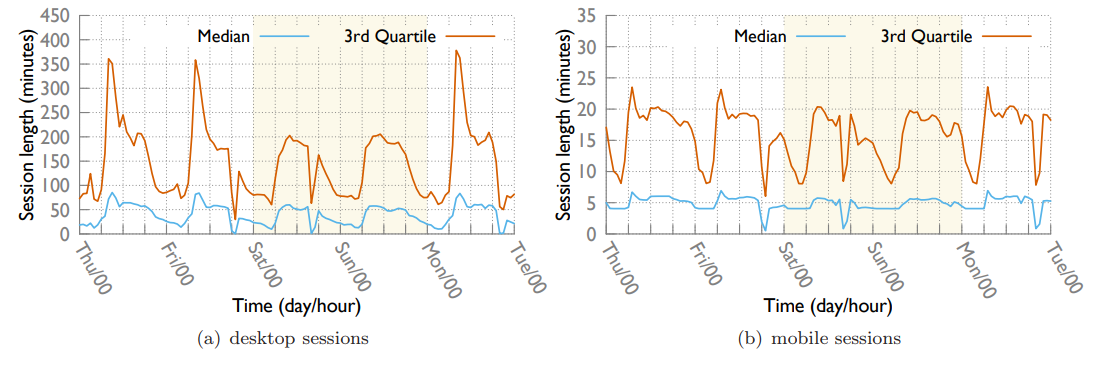
\includegraphics[height=5cm]{images/session.png}
\end{center}

The above graphs, using the same data, show that on average, mobile sessions
are shorter than their desktop companions. In addition, the morning peak is not
as pronounced, and there is more overall variation. Since these graphs suggest
a difference in listening habits between mobile and desktop, reflecting these
practices in Scottipy is an intriguing task. Since desktop sessions tend to
be longer, it may be fruitful to increase the default number of songs generated
for the platform. On mobile, it would be worthwhile to investigate tailoring
the list to shorter playlists, perhaps by involving song popularity, or other
efforts that could simultaneously lower the amount of music, but make each track
more meaningfully chosen by the data metrics Spotify gives.

\section{Conclusion}
The data that The Echo Nest and Spotify have aggregated makes finding new music
the easiest that it has ever been. Despite this, music discovery on the Spotify
platform is currently limited to just one weekly static playlist. The project
I have outlined will allow music listeners to harness the data that Spotify posesses,
in the hopes of finding unfamiliar but enjoyable music. This project aims to make
music discovery a more easy and rewarding task than currently possible.
 % Conclusion/future work

%   ********************************************************************
%   * IF YOU HAVE ANY APPENDICES (FOR INSTANCE, CODE, DATA, GRAPHS,    *
%   * OR ANYTHING ELSE THAT DOESN'T "FIT" AS REGULAR CHAPTER CONTENT), *
%   * INCLUDE THE FOLLOWING LINE, WHICH INSTRUCTS LATEX TO CHANGE FROM *
%   * NUMBERED "CHAPTER" HEADINGS TO LETTERED "APPENDIX" HEADINGS.     *
%   *                                                                  *
%   * APPENDICES HAVE THE SAME FORMATTING COMMANDS AS CHAPTERS (E.G.,  *
%   * "\chapter{...}", "\section{...}", ETC.)                          *
%   ********************************************************************

\appendix

% $Id: appa--code
%
%   *******************************************************************
%   * SEE THE MAIN FILE "AllegThesis.tex" FOR MORE INFORMATION.       *
%   *******************************************************************

\chapter{Python Code: \texttt{main.py}}\label{appa:srccode}

%   *******************************************************************
%   * SEE THE MAIN FILE "AllegThesis.tex" FOR THE "\lstset" COMMAND   *
%   * THAT DEFINES HOW PROGRAM LISTINGS WILL LOOK.                    *
%   *******************************************************************

\lstinputlisting{src/main.py}
  % Appendices go here

% $Id: appa--code
%
%   *******************************************************************
%   * SEE THE MAIN FILE "AllegThesis.tex" FOR MORE INFORMATION.       *
%   *******************************************************************

\chapter{Python Code: \texttt{recent.py}}\label{appa:srccode}

%   *******************************************************************
%   * SEE THE MAIN FILE "AllegThesis.tex" FOR THE "\lstset" COMMAND   *
%   * THAT DEFINES HOW PROGRAM LISTINGS WILL LOOK.                    *
%   *******************************************************************

\lstinputlisting{src/recent.py}


% $Id: appa--code
%
%   *******************************************************************
%   * SEE THE MAIN FILE "AllegThesis.tex" FOR MORE INFORMATION.       *
%   *******************************************************************

\chapter{Python Code: \texttt{edit.py}}\label{appa:srccode}

%   *******************************************************************
%   * SEE THE MAIN FILE "AllegThesis.tex" FOR THE "\lstset" COMMAND   *
%   * THAT DEFINES HOW PROGRAM LISTINGS WILL LOOK.                    *
%   *******************************************************************

\lstinputlisting{src/edit.py}


% $Id: appa--code
%
%   *******************************************************************
%   * SEE THE MAIN FILE "AllegThesis.tex" FOR MORE INFORMATION.       *
%   *******************************************************************

\chapter{HTML Templates}\label{appa:htmlcode}

%   *******************************************************************
%   * SEE THE MAIN FILE "AllegThesis.tex" FOR THE "\lstset" COMMAND   *
%   * THAT DEFINES HOW PROGRAM LISTINGS WILL LOOK.                    *
%   *******************************************************************

\section{\texttt{index.html}}
\lstinputlisting{src/templates/index.html}

\pagebreak

\section{\texttt{runRecentlyAdded.html}}

\lstinputlisting{src/templates/runRecentlyAdded.html}

\pagebreak

\section{\texttt{running.html}}

\lstinputlisting{src/templates/running.html}

\section{\texttt{success.html}}

\lstinputlisting{src/templates/success.html}


%   ********************************************************************
%   * THE FINAL COMMANDS DEAL WITH BIBLIOGRAPHY/REFERENCES. IF THERE   *
%   * ARE ANY ITEMS IN YOUR BIBTEX FILE THAT YOU DID NOT REFERENCE IN  *
%   * YOUR PAPER, BUT THAT YOU WISH TO INCLUDE IN THE BIBLIOGRAPHY,    *
%   * YOU MAY SPECIFY "\nocite" COMMANDS TO FORCE THEM TO BE INCLUDED. *
%   *                                                                  *
%   * THE COMMAND "\nocite{*}" FORCES EVERY ITEM IN YOUR BIBTEX FILE.  *
%   ********************************************************************

%\nocite{ckm-acmap-99}   % EXAMPLES OF FORCING THINGS TO BE INCLUDED
%\nocite{Dierckx93}      %   "   "   "
%\nocite{obs-stcav-92}   %   "   "   "
%\nocite{bb4471}         %   "   "   "

\nocite{*} % OR DO THIS TO INCLUDE ALL BIBTEX REFERENCES IN THE BIBLIOGRAPHY

\bibliographystyle{plain}

%   ********************************************************************
%   * IF YOU HAVE YOUR BIBLIOGRAPHY IN A SEPARATE ".bib" FILE, HERE IS *
%   * WHERE YOU MUST SPECIFY IT. IN THIS EXAMPLE, THE BIBLIOGRAPHY     *
%   * ENTRIES ARE STORED IN A SUBDIRECTORY NAMED "Bibdir" IN A FILE    *
%   * NAMED "myBibtexDB.bib".                                          *
%   ********************************************************************

\begin{spacing}{1}
\bibliography{bibDir/bib}    % File type ".bib" is assumed
\end{spacing}

%   ********************************************************************
%   * THIS FEATURE HAS BEEN DISABLED:                                  *
%   ********************************************************************
% \include{colophon}

\typeout{THEPAGE \thepage}

\end{document}
